\subsection{HTB04 - BankRobber}

    \subsubsection{Escaneo}
        \large{Como primera etapa de la Prueba de Penetración realizamos un escaneo de puertos abiertos en la máquina víctima con la herramienta "Nmap", los hallados fueron 4, con los servicios 'http', 'ssl/http', 'microsoft ds' y 'mysql'.}
        \par
        \begin{figure}[h!]
            \centering
            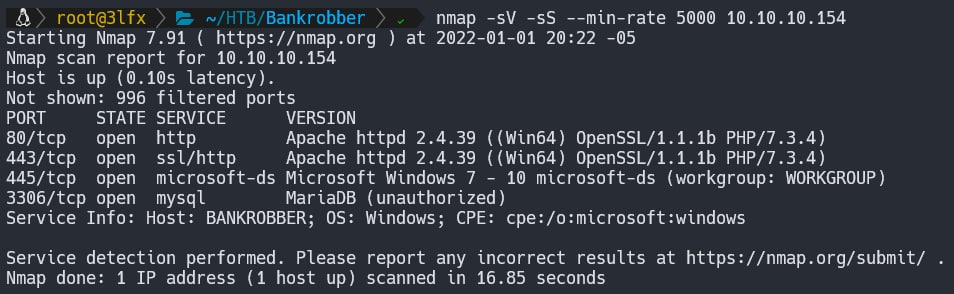
\includegraphics[width=0.99\textwidth]{informe4/imagenes/bankrobber/01_escaneo.png}
            \caption{Escaneo de puertos BankRobber} 
        \end{figure}  

    \subsubsection{Análisis de Vulnerabilidades}

    \subsubsection{Explotación}

    \subsubsection{Escalamiento de Privilegios}

    \subsubsection{Post-Explotación}

    \subsubsection{Recomendaciones de Mitigación}